\newpage
\section*{More \LaTeX\ and Technical Writing Advice}

Unnumbered itemisation (only to be used when the order of the items
does \emph{not} matter):\footnote{Use footnotes very sparingly, and
  note that footnote pointers are \emph{never} preceded by a space and
  always glued immediately \emph{behind} the punctuation, if there is
  any.}
\begin{itemize}
\item Unnumbered displayed formula:
  \[
  E = m \cdot c^2
  \]
\item Numbered displayed formula, which is cross-referenced somewhere:
  \begin{equation}
    \label{eq:emc2}
    E = m \cdot c^2
  \end{equation}
\item Formula --- the same as formula~(\ref{eq:emc2}) --- spanning
  more than one line:
  \begin{gather*}
    E \\ = m \cdot c^2
  \end{gather*}
\end{itemize}
Numbered itemisation (only to be used when the order of the items
\emph{does} matter):
\begin{enumerate}
\item First do this.
\item\label{item:that} Then do that.
\item If we are not finished, then go back to Step~\ref{item:that},
  else stop.
\end{enumerate}

Tables and elementary mathematics are typeset as exemplified in
Table~\ref{tab:maths}; see
\url{http://tug.ctan.org/info/short-math-guide/short-math-guide.pdf}
for many more details.

\begin{table}[t] % make it float to the top of a page
  \centering
  \begin{tabular}{rlc} % right left centre
    \toprule
    Topic & \LaTeX\ code & Appearance \\
    \midrule
    Greek letter & \verb|$\Theta,\Omega,\epsilon$| & $\Theta,\Omega,\epsilon$ \\
    multiplication & \verb|$m \cdot n$| & $m \cdot n$ \\
    division & \verb|$\frac{m}{n}, m \div n$| & $\frac{m}{n}, m \div n$ \\
    rounding down & \verb|$\left\lfloor n \right\rfloor$| & $\left\lfloor n \right\rfloor$ \\
    rounding up & \verb|$\left\lceil n \right\rceil$| & $\left\lceil n \right\rceil$ \\
    binary modulus & \verb|$m \bmod n$| & $m \bmod n$ \\
    unary modulus & \verb|$m \equiv n \mod \ell$| & $m \equiv n \mod \ell$ \\
    root & \verb|$\sqrt{n},\sqrt[3]{n}$| & $\sqrt{n},\sqrt[3]{n}$ \\
    exponentiation, superscript & \verb|$n^{i}$| & $n^{i}$ \\
    subscript & \verb|$n_{i}$| & $n_{i}$ \\
    overline & \verb|$\overline{n}$| & $\overline{n}$ \\
    base $2$ logarithm & \verb|$\lg n$| & $\lg n$ \\
    base $b$ logarithm & \verb|$\log_b n$| & $\log_b n$ \\
    binomial & \verb|$\binom{n}{k}$| & $\binom{n}{k}$ \\
    sum & \verb|\[\sum_{i=1}^n i\]| & $\displaystyle\sum_{i=1}^n i$ \\
    numeric comparison & \verb|$\leq,<,=,\neq,>,\geq$| & $\leq,<,=,\neq,>,\geq$ \\
    non-numeric comparison & \verb|$\prec,\nprec,\preceq,\succeq$| & $\prec,\nprec,\preceq,\succeq$ \\
    extremum & \verb|$\min,\max,+\infty,\bot,\top$| & $\min,\max,+\infty,\bot,\top$ \\
    function & \verb|$f\colon A\to B,\circ,\mapsto$| & $f\colon A\to B,\circ,\mapsto$ \\
    sequence, tuple & \verb|$\langle a,b,c \rangle$| & $\langle a,b,c \rangle$ \\
    set & \verb|$\{a,b,c\},\emptyset,\mathbb{N}$| & $\{a,b,c\},\emptyset,\mathbb{N}$ \\
    set membership & \verb|$\in,\not\in$| & $\in,\not\in$ \\
    set comprehension & \verb|$\{i \mid 1 \leq i \leq n\}$| & $\{i \mid 1 \leq i \leq n\}$ \\
    set operation & \verb|$\cup,\cap,\setminus,\times$| & $\cup,\cap,\setminus,\times$ \\
    set comparison & \verb|$\subset,\subseteq,\not\supset$| & $\subset,\subseteq,\not\supset$ \\
    logic quantifier & \verb|$\forall,\exists,\nexists$| & $\forall,\exists,\nexists$ \\
    logic connective & \verb|$\land,\lor,\neg,\Rightarrow$| & $\land,\lor,\neg,\Rightarrow$ \\
    logic & \verb|$\models,\equiv,\vdash$| & $\models,\equiv,\vdash$ \\
    miscellaneous & \verb|$\&,\#,\approx,\sim,\ell$| & $\&,\#,\approx,\sim,\ell$ \\
    dots & \verb|$\ldots,\cdots,\vdots,\ddots$| & $\ldots,\cdots,\vdots,\ddots$ \\
    dots (context-sensitive) & \verb|$1,\dots,n; 1+\dots+n$| & $1,\dots,n; 1+\dots+n$ \\
    parentheses (autosizing) & \verb|$\left(m^{n^k}\right),(m^{n^k})$| & $\left(m^{n^k}\right),(m^{n^k})$ \\
    identifier of $>1$ character & \verb|$\mathit{identifier}$| & $\textit{identifier}$ \\
    hyphen, \emph{n}-dash, \emph{m}-dash, minus & \verb|-|, \verb|--|, \verb|---|, \verb|$-$| & -, --, ---, $-$ \\
    \bottomrule
  \end{tabular}
  \caption{The typesetting of elementary mathematics.  Note very carefully
    when italics are used by \LaTeX\ and when not, as well as all the
    horizontal and vertical spacing performed by \LaTeX.}
  \label{tab:maths}
\end{table}

Use \verb|\mathit{...}| in mathematical mode for each multiple-letter
identifier in order to avoid typesetting the identifier like the
product of single-letter ones.  For example, note the typographic
difference between the identifier $\mathit{WL}$, obtained through
\verb|$\mathit{WL}$|, and the product $WL$, where there is a small
space between the $W$ and the $L$, obtained through \verb|$WL$|.

Do \emph{not} use programming-language-style lower-ASCII notation
(such as $!$ for negation, $\&\&$ for conjunction, $||$ for
disjunction, and the equality sign $=$ for assignment) in algorithms
or formulas (but rather use $\neg$ or $\mathbf{not}$, $\land$ or $\&$
or $\mathbf{and}$, $\lor$ or $\mathbf{or}$, and $\gets$ or
$\coloneqq$, respectively), as this testifies to a very strong
confusion of concepts.

Figures can be imported with \verb|\includegraphics|
% (such as Figure~\ref{fig:demo})
or drawn inside the \LaTeX\ source code using the highly declarative
notation of the \texttt{tikz} package: see Figure~\ref{fig:trees} for
sample drawings.  It is perfectly acceptable in this course to include
scans or photos of drawings that were carefully done by hand.

%\begin{figure}[t] % make it float towards the top of a page
%  \centering
%  \includegraphics[height=5cm]{lulu.jpg}
%  \caption{The text under the figure}
%  \label{fig:demo}
%\end{figure}

\begin{figure}[t] % make it float to the top of a page
  \begin{center}
    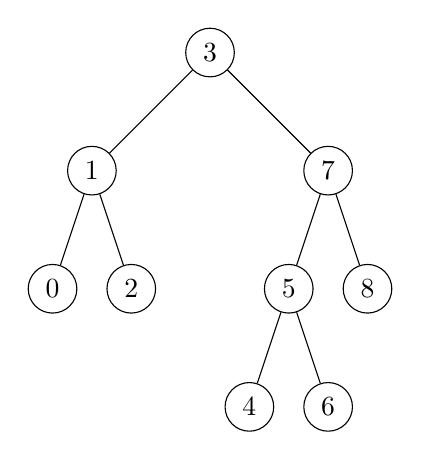
\begin{tikzpicture}
      [level 1/.style={sibling distance=30mm},
       level 2/.style={sibling distance=15mm},
       level 2/.style={sibling distance=10mm}]
      \tikzstyle{every node}=[circle,draw]
      \node{3}
      child{
        node{1}
        child{node{0}}
        child{node{2}}
      }
      child{
        node{7}
        child{
          node{5}
          child{node{4}}
          child{node{6}}
        }
        child{node{8}}
      };
    \end{tikzpicture} \hspace{4mm}
    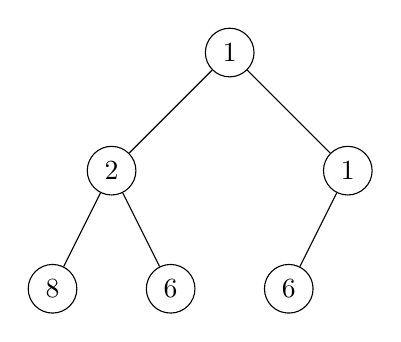
\begin{tikzpicture}
      [level 1/.style={sibling distance=30mm},
       level 2/.style={sibling distance=15mm}]
      \tikzstyle{every node}=[circle,draw]
      \node{1}
      child{
        node{2}
        child{node{8}}
        child{node{6}}
      }
      child{
        node{1}
        child{node{6}}
        child[missing]{node{k}}
      }
      ;
    \end{tikzpicture} \hspace{4mm}
    \begin{tikzpicture}[grow via three points={%
        one child at (0,-1.5) and two children at (0,-1.5) and (-1.5,-1.5)}]
      \tikzstyle{every node}=[circle,draw]
      \node at (0,0) {6}
      child{node{29}}
      child{
        node{14}
        child{
          node{38}
        }
      }
      child{
        node{8}
        child{node{17}}
        child{
          node{11}
          child{node{27}}
        }
      }
      ;
    \end{tikzpicture}
  \end{center}
  \caption{A binary search tree (on the left), a binary min-heap (in
    the middle), and a binomial tree of rank $3$ (on the right).}
  \label{fig:trees}
\end{figure}

Algorithms can be typeset as pseudo-code as exemplified in
Algorithm~\ref{algo:demo}: study its \LaTeX\ source code.

\begin{algorithm}[t]
  \begin{algorithmic}[1]  % comment [1] away to drop the line numbers
    \STATE \Function $f(n)$
    \IF[optional comment]{$n < 0$}
      \STATE $n \IsAssigned -2 \cdot n$ \COMMENT{optional comment}
    \ELSE[$n \geq 0$]
      \STATE $n \IsAssigned  3 \cdot n$
    \ENDIF
    \WHILE[optional comment]{$n > 0$}
      \STATE $n \IsAssigned n-1$
    \ENDWHILE
    \RETURN $n$
  \end{algorithmic}
  \caption{Silly algorithm}
  \label{algo:demo}
\end{algorithm}

If you are not sure whether you will stick to your current choice of
notation or terminology, then introduce a new (possibly parametric)
command.  For example, upon
\begin{center}
  \verb|\newcommand{\Cardinality}[1]{\left\lvert#1\right\rvert}|
\end{center}
the formula \verb|$\Cardinality{S}$| typesets the cardinality of set
$S$ as $\Cardinality{S}$ with autosized vertical bars and proper
spacing, but upon changing the definition of that parametric command
to
\begin{center}
  \verb|\newcommand{\Cardinality}[1]{\# #1}|
\end{center}
and recompiling, the formula \verb|$\Cardinality{S}$| typesets the
cardinality of set $S$ as $\#S$.
%
Similarly, upon
\begin{center}
  \verb|\newcommand{\MiniZinc}{\textit{Mini\-Zinc}}|
\end{center}
the text \verb|\MiniZinc\| typesets into \textit{MiniZinc},
hyphenation being only possible in the middle, but upon changing the
definition of that non-parametric command to
\begin{center}
  \verb|\newcommand{\MiniZinc}{\textsc{Mini\-Zinc}}|
\end{center}
and recompiling, the text \verb|\MiniZinc\| typesets into
\textsc{MiniZinc}.
%
You can thus obtain an arbitrary number of changes in the document
with a \emph{constant}-time change in its source code, rather than
having to perform a \emph{linear}-time find-and-replace operation
within the source code, which is painstaking and error-prone.  The
imported file \texttt{macros.tex} has a lot of useful predefined
commands about mathematics, CP, \Gecode, modelling, \MiniZinc, and
algorithms.

Use commands on positioning (such as \verb|\hspace|, \verb|\vspace|,
and \verb|\noindent|) and appearance (such as \verb|\small| for
reducing the font size, and \verb|\textit| for italics) very
sparingly, and ideally only in (parametric) commands, as the very idea
of mark-up languages such as \LaTeX\ is to let the class designer
(usually a trained professional typesetter) decide on where things
appear and how they look.  For example, \verb|\emph| (for emphasis)
compiles (outside italicised environments, such as \texttt{theorem})
into \textit{italics} under the \texttt{article} class used for this
document, but it may compile into \textbf{boldface} under some other
class.
\begin{center}
  \textbf{If you do not (need to) worry about \emph{how} things look, \\
    then you can fully focus on \emph{what} you are trying to
    express!}
\end{center}

Note that \emph{no} absolute numbers are used in the \LaTeX\ source
code for any of the references inside this document.  For ease of
maintenance, \verb|\label| is used for giving a label to something
that is automatically numbered (such as an algorithm, equation,
figure, footnote, item, line, part, section, subsection, or table),
and \verb|\ref| is used for referring to a label.  An item in the
bibliography file is referred to by \verb|\cite| instead.  Upon
changing the text, it suffices to recompile, once or twice, and
possibly to run BibTeX again, in order to update all references
consistently.

Always write
%
\verb| Table|$\sim$\verb|\ref{tab:maths} |
%
instead of
%
\verb| Table \ref{tab:maths}|,
%
by using the non-breaking space (which is typeset as the tilde $\sim$)
instead of the normal space, because this avoids that a
cross-reference is spread across a line break, as for example in
``Table \ref{tab:maths}'', which is considered poor typesetting.

The rules of English for how many spaces to use before and after
various symbols are given in Table~\ref{tab:spacing}.  Beware that
they may be very different from the rules in your native language.

\begin{table}[t]
  \centering
  \begin{tabular}{cc|c|c}
    \toprule
    \multicolumn{2}{c}{} & \multicolumn{2}{l}{number of spaces after} \\
    \cmidrule{3-4}
    \multicolumn{2}{c}{} & 0 & 1 \\
    \midrule
    \multirow{2}{*}{number of spaces before} & 0 & / - & , : ; . ! ?
    ) ] \} ' '' \% \\
    \cmidrule{2-4}
    & 1 & ( [ \{ ` `` & -- (\emph{n}-dash) --- (\emph{m}-dash) \\
    \bottomrule
  \end{tabular}
  \caption{Spacing rules of English}
  \label{tab:spacing}
\end{table}

\vfill

\noindent
\handpoint\ Feel free to report to the head teacher any other features
that you would have liked to see discussed and exemplified in this
template document.
